\documentclass[../main.tex]{subfiles}
\begin{document}
%=========================================================
% TĐ_GiaoAn_IQB_HK1_Tuan06_OnTapPhepNhan_ToanLoiVan
% Giáo án Toán tư duy cấp độ B
%   Buổi 1: ÔN TẬP PHÉP NHÂN (90 phút)
%   Buổi 2: TOÁN CÓ LỜI VĂN -- PHÉP CỘNG, PHÉP TRỪ (90 phút)
% Soạn theo mẫu (\hktuan, \subsection, hd, vd, luuy)
% Hình đặt trong thư mục Hinh_GiaoAn_Tuan06/ (cùng cấp với file này), tên hình có tiền tố ga06_
\graphicspath{{Hinh_GiaoAn_Tuan06/}{Data_GiaoAn_HK0/Hinh_GiaoAn_Tuan06/}}
%=========================================================

%---------- Màu dùng riêng cho giáo án ----------
\definecolor{gaTim}{HTML}{5A3EA8}     % mực tím (vở HS)
\definecolor{gaDo}{HTML}{C4313A}      % bút đỏ GV
\definecolor{gaXanhLa}{HTML}{3F8A4F}
\definecolor{gaCam}{HTML}{E08A1E}
\definecolor{gaBang}{HTML}{23453A}    % bảng đen (xanh)
\definecolor{gaGo}{HTML}{8A5A2B}      % khung gỗ
\definecolor{gaPhanVang}{HTML}{F5DC78}
\definecolor{gaPhanHong}{HTML}{F4A9B8}
\definecolor{gaPhanXanh}{HTML}{A9DCF0}
\definecolor{gaBangGiay}{HTML}{4F86C6}
\definecolor{gaT1}{HTML}{2F7F9E}\definecolor{gaT2}{HTML}{5A3EA8}\definecolor{gaT3}{HTML}{D07A1F}
\definecolor{gaT4}{HTML}{3F8A4F}\definecolor{gaT5}{HTML}{C4313A}\definecolor{gaT6}{HTML}{6B7A72}

%---------- Lệnh dùng riêng cho giáo án ----------
% Chèn hình căn giữa, dính liền với đoạn phía trên; tham số = chiều cao tối đa
\providecommand{\TThinh}{}\renewcommand{\TThinh}[2][8cm]{\par\nopagebreak\vspace{2pt}\nopagebreak{\centering\includegraphics[height=#1,width=\linewidth,keepaspectratio]{#2}\par}\vspace{2pt}}
% Chỗ chấm điền
\providecommand{\TTcham}[1][3cm]{\makebox[#1]{\dotfill}}
% Chú thích hình
\providecommand{\GAchuthich}{}\renewcommand{\GAchuthich}[1]{\par\nopagebreak{\centering\small\textit{#1}\par}\medskip}
% Tiêu đề mục nhỏ trong một hoạt động
\providecommand{\GAmucnho}{}\renewcommand{\GAmucnho}[1]{\par\addvspace{4pt}\noindent{\color{mauchinh}\bfseries #1}\par\nopagebreak\addvspace{2pt}}
% Lời GV nói với HS (in nghiêng, có dấu ngoặc kép)
\providecommand{\GAloi}{}\renewcommand{\GAloi}[1]{\textit{“#1”}}
% Đáp án gợi ý cho GV (chữ xám)
\providecommand{\GAdapan}{}\renewcommand{\GAdapan}[1]{\textcolor{black!55}{(#1)}}
% Khung chốt kiến thức
\providecommand{\GAchot}{}\renewcommand{\GAchot}[1]{\par\smallskip\noindent\fcolorbox{mauchinh}{white}{\parbox{\dimexpr\linewidth-2\fboxsep-2\fboxrule\relax}{#1}}\par\smallskip}
% Thẻ từ khóa: \GAchip{màu}{chữ}
\providecommand{\GAchip}{}\renewcommand{\GAchip}[2]{\tikz[baseline=(c.base)]\node(c)[draw=#1,text=#1,rounded corners=6pt,inner xsep=5pt,inner ysep=2pt,font=\small]{#2};}
% Bài trình bày trong vở ô li: \GAvo{dòng 1\\ dòng 2\\ ...}
\newsavebox{\GAvohop}\newlength{\GAvocao}
\providecommand{\GAvo}{}\renewcommand{\GAvo}[1]{\par\smallskip\noindent
  \sbox{\GAvohop}{\parbox{\dimexpr\linewidth-24pt\relax}{\color{gaTim}\fontsize{12.5pt}{8mm}\selectfont\itshape #1}}%
  \setlength{\GAvocao}{\ht\GAvohop}\addtolength{\GAvocao}{\dp\GAvohop}\addtolength{\GAvocao}{10pt}%
  \begin{tikzpicture}
    \fill[gaTim!2] (0,0) rectangle (\linewidth-0.8pt,\GAvocao);
    \begin{scope}
      \clip (0,0) rectangle (\linewidth-0.8pt,\GAvocao);
      \draw[gaTim!12,line width=0.3pt] (0,0) grid[xstep=8mm,ystep=2mm] (\linewidth,\GAvocao);
      \draw[gaTim!32,line width=0.4pt] (0,0) grid[xstep=8mm,ystep=8mm] (\linewidth,\GAvocao);
    \end{scope}
    \draw[gaTim!45] (0,0) rectangle (\linewidth-0.8pt,\GAvocao);
    \node[anchor=south west,inner sep=0pt] at (12pt,5pt) {\usebox{\GAvohop}};
  \end{tikzpicture}\par\smallskip}
% Thanh thời lượng 90 phút: \GAthoigian{bắt đầu/số phút/nhãn/màu, ...}
\newlength{\GAphut}
\providecommand{\GAthoigian}{}\renewcommand{\GAthoigian}[1]{\par\smallskip\noindent
  \setlength{\GAphut}{\linewidth}\addtolength{\GAphut}{-4pt}\divide\GAphut by 90
  \begin{tikzpicture}[x=\GAphut,y=1cm]
    \foreach \bd/\sp/\nhan/\mau in {#1}{
      \fill[\mau] (\bd,0) rectangle (\bd+\sp,0.62);
      \draw[white,line width=1.5pt] (\bd+\sp,0) -- (\bd+\sp,0.62);
      \node[white,font=\scriptsize\bfseries] at (\bd+\sp/2,0.31) {\nhan};
    }
  \end{tikzpicture}\par\smallskip}
% Một ô thẻ số
\providecommand{\GAthe}{}\renewcommand{\GAthe}[3][black!25]{\node[draw=#1,fill=white,rounded corners=4pt,minimum width=1.25cm,minimum height=1.5cm,font=\huge\bfseries,text=mauchinh] at #2 {#3};}

%%%%%%%%%%%%%%%%%%%%%%%%%%%%%%%%%%%%%%%%%%%%%%%%%%%%%%%%%%
%                       BUỔI 1
%%%%%%%%%%%%%%%%%%%%%%%%%%%%%%%%%%%%%%%%%%%%%%%%%%%%%%%%%%
%\setcounter{section}{3} % không chỉnh sửa
\hktuan{1}{6}
\par\medskip
%\textbf{Người soạn: }
\begin{center}
        {\color{mauchinh!120}\bfseries\Large ÔN TẬP PHÉP NHÂN (BUỔI 1)}
\end{center}

\subsection{MỤC TIÊU CẦN ĐẠT}
\begin{itemize}
    \item \textbf{Kiến thức:} HS nhắc lại được ý nghĩa phép nhân: $a \times b$ là $a$ được lấy $b$ lần (tổng của $b$ số hạng, mỗi số hạng bằng $a$); gọi đúng tên \textbf{thừa số}, \textbf{tích}.
    \item \textbf{Kiến thức:} HS nắm chắc quy tắc nhân với 1, nhân với 0 và tính chất giao hoán $a \times b = b \times a$.
    \item \textbf{Kỹ năng:} HS thuộc bảng nhân 2 -- 9; viết được phép nhân từ hình ảnh; so sánh hai tích mà không cần tính; giải được bài toán tăng, giảm thừa số.
    \item \textbf{Kỹ năng:} HS trình bày đúng bài toán có lời văn một phép nhân (thừa số thứ nhất cùng đơn vị với kết quả).
    \item \textbf{Năng lực:} HS giải thích bằng lời vì sao chọn phép tính, vì sao điền dấu; hợp tác trong nhóm 2 -- 3 bạn.
    \item \textbf{Phẩm chất:} HS tập trung, cẩn thận, trình bày vở sạch đẹp.
\end{itemize}

\subsection{TIẾN TRÌNH DẠY HỌC}
\textbf{Đồ dùng dạy học:} giáo án, PBT, sách Titan, bảng con, phấn màu, nam châm, con dấu, sticker; thẻ số (0 -- 9, dấu $\times$, dấu $=$); tranh “Đĩa cam”, “Khay trứng”, “Lốc sữa”, “Lọ hoa”; 1 lốc sữa thật (hoặc vỏ hộp); mô hình cân đĩa (nếu có).

\begin{luuy}
    \textbf{Cách tính điểm cả buổi -- “Giỏ cam”:} mỗi đội có một giỏ cam vẽ trên bảng. Trả lời đúng, giải thích hay, làm nhanh được gắn thêm một quả cam nam châm. Cuối buổi đội nhiều cam nhất được tặng sticker.
\end{luuy}

\GAmucnho{Phân bố thời gian (90 phút)}
\GAthoigian{0/10/HĐ1: 10 ph/gaT1, 10/20/HĐ2: 20 ph/gaT2, 30/10/HĐ3: 10 ph/gaT3, 40/20/HĐ4: 20 ph/gaT4, 60/20/HĐ5: 20 ph/gaT5, 80/10/HĐ6: 10 ph/gaT6}
{\small HĐ1: Khởi động \quad HĐ2: Ý nghĩa phép nhân \quad HĐ3: Thành phần, nhân với 1, nhân với 0 \quad HĐ4: So sánh, tăng giảm thừa số \quad HĐ5: Toán lời văn \quad HĐ6: Củng cố\par}

\GAmucnho{Trình bày bảng lớp (cố định suốt 90 phút)}
\begin{center}
\begin{tikzpicture}
\node[fill=gaBang,draw=gaGo,line width=5pt,rounded corners=2pt,inner sep=7pt,text=white]{%
\renewcommand{\arraystretch}{1.25}%
\begin{tabular}{p{0.37\linewidth}!{\color{white!45}\vrule}p{0.29\linewidth}!{\color{white!45}\vrule}p{0.16\linewidth}}
    {\color{gaPhanVang}\bfseries\underline{Ghi nhớ}} & {\color{gaPhanVang}\bfseries\underline{Ví dụ mẫu}} & {\color{gaPhanVang}\bfseries\underline{Luyện tập}} \\
    1. $a \times b = \underbrace{a + a + \dots + a}_{b\ \mbox{số hạng}}$ & $3+3+3+3+3 = 15$ & {\small\color{white!70} HS lên bảng làm bài; GV chữa bằng phấn màu.} \\
    2. {\color{gaPhanHong}Thừa số} $\times$ {\color{gaPhanHong}Thừa số} $=$ {\color{gaPhanVang}Tích} & $\Rightarrow$ {\color{gaPhanVang}$3 \times 5 = 15$} (quả) & \\
    3. $a \times b = b \times a$ & $15 \times 4 < 15 \times 6$ vì $4 < 6$ & \\
    \quad $a \times 1 = a$ \quad $a \times 0 = 0$ & $4 \times 6 = 24 \to 4 \times 9 = 36$ & \\
    4. {\color{gaPhanHong}Tích tăng = TS thứ nhất $\times$ số đơn vị tăng} & Tích tăng: {\color{gaPhanXanh}$4 \times 3 = 12$} & \\
\end{tabular}};
\end{tikzpicture}
\end{center}

%---------------------------------------------------------
\subsubsection{KHỞI ĐỘNG -- SỬA BÀI TẬP VỀ NHÀ}
\begin{hd}
    \begin{itemize}
        \item Thời gian: 10 phút
        \item Tạo không khí sôi nổi; kiểm tra nhanh bảng nhân; rút kinh nghiệm lỗi sai ở BTVN.
    \end{itemize}
\end{hd}
\GAmucnho{Trò chơi “Truyền điện bảng nhân” (5 phút)}
\begin{itemize}
    \item GV nói một phép nhân, ví dụ \GAloi{$3 \times 4$}, và chỉ vào một HS. HS trả lời \GAloi{12}, rồi tự nêu một phép nhân khác và “truyền điện” cho bạn tiếp theo.
    \item Bạn trả lời sai hoặc quá 5 giây thì làm một động tác vui (vỗ tay 3 cái, nhảy tại chỗ) rồi chơi tiếp, không bị loại.
    \item Vòng 2 tăng độ khó: chỉ được nêu phép nhân trong bảng 6, 7, 8, 9.
\end{itemize}
\GAmucnho{Sửa BTVN: “Thám tử bắt lỗi” (5 phút)}
\begin{itemize}
    \item GV chữa nhanh 4 bài tập trong phiếu tự luyện. Chiếu 2 bài có lỗi sai (che tên HS) và hỏi: \GAloi{Thám tử nào tìm ra lỗi sai?}
    \item Tuyên dương HS đạt điểm 10; nhắc lỗi tính nhẩm cẩu thả, viết ngược thứ tự thừa số.
\end{itemize}

%---------------------------------------------------------
\subsubsection{“ĐI CHỢ CÙNG BÀ” -- ÔN Ý NGHĨA PHÉP NHÂN}
\begin{hd}
    \begin{itemize}
        \item Thời gian: 20 phút
        \item HS viết được phép cộng các số hạng bằng nhau và phép nhân tương ứng từ hình ảnh; xác định đúng thừa số thứ nhất (số lượng của một nhóm) và thừa số thứ hai (số nhóm).
    \end{itemize}
\end{hd}
\GAmucnho{a) Những đĩa cam của bà}
GV dẫn chuyện: \GAloi{Sáng nay bà đi chợ mua cam về bày lên bàn thờ ngày rằm. Bà bày thành từng đĩa như thế này.} GV treo Hình 1.
\TThinh[2.4cm]{ga06_diacam.png}
\GAchuthich{Hình 1. Bà bày 5 đĩa cam, mỗi đĩa 3 quả.}
\begin{itemize}
    \item \GAloi{Mỗi đĩa có mấy quả cam?} \hfill (3 quả)
    \item \GAloi{Có mấy đĩa như thế?} \hfill (5 đĩa)
    \item \GAloi{Muốn biết có tất cả bao nhiêu quả, con viết phép cộng thế nào?} \hfill ($3+3+3+3+3 = 15$)
    \item \GAloi{Số 3 được lấy mấy lần?} \hfill (5 lần, ta viết $3 \times 5 = 15$)
\end{itemize}
\GAchot{\textbf{Chốt:} Thừa số thứ nhất là số lượng của \textbf{một nhóm} (3 quả trong một đĩa). Thừa số thứ hai là \textbf{số nhóm} (5 đĩa). Vì vậy viết $3 \times 5$, không viết $5 \times 3$.}

\GAmucnho{b) Khay trứng -- đếm theo hàng và theo cột}
\TThinh[4.2cm]{ga06_khaytrung.png}
\GAchuthich{Hình 2. Khay trứng gà: vòng đỏ là một hàng (5 quả), vòng tím là một cột (2 quả).}
\begin{itemize}
    \item GV khoanh hàng 1 bằng phấn đỏ: \GAloi{Mỗi hàng mấy quả? Có mấy hàng?} \hfill ($5 \times 2 = 10$)
    \item GV khoanh cột 1 bằng phấn tím: \GAloi{Mỗi cột mấy quả? Có mấy cột?} \hfill ($2 \times 5 = 10$)
    \item \GAloi{Số trứng trong khay có thay đổi không?} \GAdapan{Không, vẫn là 10 quả. Vậy $5 \times 2 = 2 \times 5$}
\end{itemize}
\GAchot{\textbf{Tính chất giao hoán:} Khi đổi chỗ các thừa số thì tích không thay đổi: $a \times b = b \times a$.}

\GAmucnho{Luyện tập trong PBT: Bài 1, Bài 2}
\textbf{Bài 1.} Quan sát hình, viết phép cộng rồi viết phép nhân thích hợp.
\begin{enumerate}[a)]
    \item Mẹ mua 3 lốc sữa, mỗi lốc 4 hộp.
    \TThinh[1.9cm]{ga06_locsua.png}
    \TTcham[1.5cm] $+$ \TTcham[1.5cm] $+$ \TTcham[1.5cm] $=$ \TTcham[1.5cm] $\Rightarrow$ \TTcham[1.5cm] $\times$ \TTcham[1.5cm] $=$ \TTcham[1.5cm] \hfill \GAdapan{$4+4+4=12$; $4 \times 3 = 12$}
    \item Cô bày 4 lọ hoa, mỗi lọ 5 bông.
    \TThinh[3cm]{ga06_lohoa.png}
    \TTcham[1.5cm] $+$ \TTcham[1.5cm] $+$ \TTcham[1.5cm] $+$ \TTcham[1.5cm] $=$ \TTcham[1.5cm] $\Rightarrow$ \TTcham[1.5cm] $\times$ \TTcham[1.5cm] $=$ \TTcham[1.5cm] \hfill \GAdapan{$5 \times 4 = 20$}
\end{enumerate}
\begin{luuy}
    Lỗi hay gặp, GV chú ý sửa ngay:
    \begin{itemize}
        \item HS viết $3 \times 4$ cho câu a) vì “có 3 lốc” $\Rightarrow$ hỏi lại: \GAloi{Số nào cho biết một lốc có mấy hộp? Số đó đứng trước.}
        \item Cho HS cầm lốc sữa thật, đếm từng hộp trong một lốc rồi đếm số lốc. Cách này giúp HS nhớ lâu hơn.
    \end{itemize}
\end{luuy}

\textbf{Bài 2 (PBT).} Nối mỗi tổng với phép nhân thích hợp. \GAdapan{$2+2+2 \to 2 \times 3$; $5+5+5+5 \to 5 \times 4$; $3+3 \to 3 \times 2$; $6+6+6 \to 6 \times 3$; $4+4+4+4 \to 4 \times 4$}

%---------------------------------------------------------
\subsubsection{THÀNH PHẦN PHÉP NHÂN -- NHÂN VỚI 1, NHÂN VỚI 0}
\begin{hd}
    \begin{itemize}
        \item Thời gian: 10 phút
        \item HS gọi đúng tên thừa số, tích; vận dụng nhanh quy tắc nhân với 1 và nhân với 0.
    \end{itemize}
\end{hd}
\GAmucnho{a) “Gắn nhãn cho phép nhân”}
GV gắn thẻ số $7 \times 3 = 21$ lên bảng, mời HS lên gắn nhãn tên gọi dưới mỗi số.
\begin{center}
\begin{tikzpicture}
    \GAthe{(0,0)}{7}
    \node[font=\huge] at (1.15,0) {$\times$};
    \GAthe{(2.3,0)}{3}
    \node[font=\huge] at (3.45,0) {$=$};
    \node[draw=black!25,fill=white,rounded corners=4pt,minimum width=1.6cm,minimum height=1.5cm,font=\huge\bfseries,text=mauchinh] at (4.75,0) {21};
    \foreach \x/\ten in {0/Thừa số, 2.3/Thừa số, 4.75/Tích}{
        \draw[gaDo,->,>=stealth,thick] (\x,-1.45) -- (\x,-0.85);
        \node[gaDo,font=\bfseries] at (\x,-1.75) {\ten};
    }
\end{tikzpicture}
\end{center}
GV nhấn mạnh: \GAloi{Cả phép tính $7 \times 3$ cũng được gọi là tích.}

\GAmucnho{b) Nhân với 1 và nhân với 0}
\begin{itemize}
    \item \GAloi{Bà chỉ bày 1 đĩa cam, mỗi đĩa 3 quả. Có mấy quả?} \GAdapan{$3 \times 1 = 3$. Số nào nhân với 1 cũng bằng chính số đó}
    \item GV treo Hình 3: \GAloi{Các con ăn hết cam rồi, còn lại 4 cái đĩa. Mỗi đĩa có mấy quả?} \GAdapan{0 quả. $0+0+0+0 = 0$, nên $0 \times 4 = 0$}
\end{itemize}
\TThinh[1.2cm]{ga06_diatrong.png}
\GAchuthich{Hình 3. 4 cái đĩa, mỗi đĩa 0 quả: $0 \times 4 = 0$.}
\GAchot{\centering $a \times 1 = 1 \times a = a$ \qquad\qquad $a \times 0 = 0 \times a = 0$}
\begin{vd}
    Bảng con nhanh (HS viết kết quả, giơ bảng cùng lúc):
    \begin{multicols}{4}
    \begin{enumerate}
        \item $9 \times 1 =$ \dots \hfill (9)
        \item $1 \times 8 =$ \dots \hfill (8)
        \item $6 \times 0 =$ \dots \hfill (0)
        \item $0 \times 7 =$ \dots \hfill (0)
    \end{enumerate}
    \end{multicols}
\end{vd}

\GAmucnho{Luyện tập trong PBT: Bài 3, Bài 4}
\begin{itemize}
    \item \textbf{Bài 3:} viết thừa số, tích vào bảng; hai dòng cuối HS tự viết phép nhân từ hai thừa số cho sẵn. \GAdapan{$8 \times 2 = 16$; $5 \times 6 = 30$}
    \item \textbf{Bài 4:} tính nhẩm 16 phép nhân trong bảng 2 -- 9, có nhân với 1 và nhân với 0. HS đổi phiếu chấm chéo.
\end{itemize}

%---------------------------------------------------------
\subsubsection{“CHIẾC CÂN KÌ DIỆU” -- SO SÁNH KHÔNG CẦN TÍNH, TĂNG GIẢM THỪA SỐ}
\begin{hd}
    \begin{itemize}
        \item Thời gian: 20 phút
        \item HS so sánh hai tích có một thừa số bằng nhau mà không cần tính; tìm được tích tăng (giảm) bao nhiêu khi một thừa số thay đổi.
    \end{itemize}
\end{hd}
\GAmucnho{a) So sánh không cần tính}
\TThinh[4.6cm]{ga06_candia.png}
\GAchuthich{Hình 4. Cân nghiêng về phía $15 \times 6$, vì 15 được lấy 6 lần nhiều hơn 15 được lấy 4 lần.}
GV phân tích mẫu theo 3 bước:
\begin{itemize}
    \item \textbf{Bước 1.} Tìm thừa số giống nhau: cả hai vế đều có thừa số 15.
    \item \textbf{Bước 2.} So sánh thừa số còn lại: $4 < 6$.
    \item \textbf{Bước 3.} Kết luận: $15 \times 4 < 15 \times 6$ (không cần tính ra 60 và 90).
\end{itemize}
\GAchot{\textbf{Quy tắc:} Hai tích có một thừa số bằng nhau, tích nào có thừa số còn lại lớn hơn thì tích đó lớn hơn.}
\textbf{Bài 5 (PBT).} Điền dấu $>$, $<$, $=$ vào chỗ chấm. HS phải giải thích bằng lời: \GAloi{Vì sao con điền dấu đó mà không cần tính?}
\begin{multicols}{2}
\begin{enumerate}[a)]
    \item $4 \times 5$ \dots\ $5 \times 4$ \hfill ($=$, giao hoán)
    \item $7 \times 6$ \dots\ $7 \times 8$ \hfill ($<$ vì $6 < 8$)
    \item $13 \times 3$ \dots\ $12 \times 3$ \hfill ($>$ vì $13 > 12$)
    \item $5+5+5+5$ \dots\ $5 \times 3$ \hfill ($>$ vì vế trái là $5 \times 4$)
    \item $9 \times 0$ \dots\ $1 \times 0$ \hfill ($=$, đều bằng 0)
    \item $8 \times 1$ \dots\ $8 + 1$ \hfill ($<$ vì $8 < 9$)
\end{enumerate}
\end{multicols}

\textbf{Bài 6 (PBT).} Trong mỗi cặp, khoanh vào phép nhân có tích lớn hơn. Lưu ý câu d) $7 \times 5$ và $5 \times 8$: HS đổi $7 \times 5 = 5 \times 7$ rồi mới so sánh.

\GAmucnho{b) “Thẻ số của Pi” -- tích tăng bao nhiêu?}
\begin{center}
\begin{tikzpicture}
    \GAthe{(0,0)}{4}
    \node[font=\huge] at (1.05,0) {$\times$};
    \GAthe{(2.1,0)}{6}
    \node[font=\huge] at (3.15,0) {$=$};
    \node[draw=black!25,fill=white,rounded corners=4pt,minimum width=1.6cm,minimum height=1.5cm,font=\huge\bfseries,text=mauchinh] at (4.35,0) {24};
    \draw[thick,->,>=stealth] (5.45,0) -- (6.35,0);
    \GAthe{(7.3,0)}{4}
    \node[font=\huge] at (8.35,0) {$\times$};
    \node[draw=gaCam,line width=1.2pt,fill=gaCam!8,rounded corners=4pt,minimum width=1.25cm,minimum height=1.5cm,font=\huge\bfseries,text=gaDo,rotate=-7] at (9.4,0) {9};
    \node[font=\huge] at (10.45,0) {$=$};
    \node[draw=black!40,dashed,fill=white,rounded corners=4pt,minimum width=1.25cm,minimum height=1.5cm,font=\huge\bfseries,text=black!40] at (11.5,0) {?};
    \draw[gaDo,thick,dashed,->,>=stealth] (2.1,0.9) to[bend left=22] node[above,font=\small\itshape]{lật ngược thẻ 6 thành 9} (9.4,0.95);
\end{tikzpicture}
\end{center}
\GAchuthich{Hình 5. Pi xếp phép nhân $4 \times 6 = 24$ bằng thẻ số, rồi vô tình lật ngược thẻ 6 thành thẻ 9.}
\textbf{Đề bài.} Pi xếp phép nhân $4 \times 6 = 24$. Do sơ ý, Pi lật ngược thẻ số 6 thành số 9.
\begin{enumerate}[a)]
    \item Phép tính mới là gì? Tính kết quả.
    \item Tích mới tăng thêm bao nhiêu đơn vị so với tích ban đầu?
\end{enumerate}
\textbf{HS trình bày vở:}
\GAvo{a) Phép tính mới: $4 \times 9 = 36$\\
b) Cách 1: Tích tăng thêm: $36 - 24 = 12$ (đơn vị)\\
\phantom{b) }Cách 2: Thừa số thứ hai tăng: $9 - 6 = 3$ (đơn vị)\\
\phantom{b) Cách 2: }Tích tăng thêm: $4 \times 3 = 12$ (đơn vị)}
GV giảng Cách 2: \GAloi{Thừa số thứ hai tăng 3 nghĩa là số 4 được lấy thêm 3 lần nữa, nên tích tăng thêm $4 \times 3 = 12$.}
\GAchot{\textbf{Công thức đóng khung vào vở:}\par\smallskip
{\centering\begin{tabular}{@{}r@{\ $=$\ }l@{}}
    Tích tăng thêm & Thừa số thứ nhất $\times$ Số đơn vị thừa số thứ hai tăng thêm\\[2pt]
    Tích giảm đi   & Thừa số thứ nhất $\times$ Số đơn vị thừa số thứ hai giảm đi
\end{tabular}\par}}

\textbf{Bài 7 (PBT)} là bài tương tự với thẻ $6 \times 4 = 24$, lật thẻ 6 thành 9 (lần này thừa số thứ nhất thay đổi). \GAdapan{$9 \times 4 = 36$; tích tăng $36 - 24 = 12$, hoặc 3 được lấy thêm 4 lần: $3 \times 4 = 12$}

\textbf{Bài 8 (PBT).}
\begin{enumerate}
    \item Một phép nhân có thừa số thứ nhất là 6, thừa số thứ hai là 5. Nếu tăng thừa số thứ hai thêm 2 đơn vị thì tích tăng thêm bao nhiêu đơn vị? \GAdapan{$6 \times 2 = 12$ đơn vị}
    \item Cho phép nhân $8 \times 5 = 40$. Nếu thay số 5 bằng số 3 thì tích tăng hay giảm bao nhiêu đơn vị? \GAdapan{giảm; $8 \times 3 = 24$, $40 - 24 = 16$, hoặc $8 \times 2 = 16$ đơn vị}
    \item \textit{(Dành cho HS giỏi)} Trong một phép nhân, nếu tăng thừa số thứ nhất thêm 3 đơn vị thì tích tăng 15 đơn vị. Tìm thừa số thứ hai. \GAdapan{thừa số thứ hai được lấy thêm 3 lần thì được 15, mà $5 \times 3 = 15$, nên thừa số thứ hai là 5}
\end{enumerate}

%---------------------------------------------------------
\subsubsection{GIẢI BÀI TOÁN CÓ LỜI VĂN BẰNG PHÉP NHÂN}
\begin{hd}
    \begin{itemize}
        \item Thời gian: 20 phút
        \item HS nhận ra “mỗi nhóm có bao nhiêu” và “có mấy nhóm”; trình bày bài giải đủ 3 phần: câu lời giải -- phép tính -- đáp số.
    \end{itemize}
\end{hd}
\begin{vd}
    Mỗi hộp có 8 chiếc bút màu. Cô giáo mua 4 hộp như thế. Hỏi cô giáo mua tất cả bao nhiêu chiếc bút màu?
\end{vd}
\TThinh[2.6cm]{ga06_hopbut.png}
\GAchuthich{Hình 6. 4 hộp bút màu, mỗi hộp 8 chiếc.}
\begin{itemize}
    \item GV hướng dẫn gạch chân từ khóa: \underline{mỗi hộp 8 chiếc}, \underline{4 hộp}, \underline{tất cả bao nhiêu chiếc}.
    \item \GAloi{Số 8 được lấy mấy lần?} \hfill (4 lần $\Rightarrow 8 \times 4$)
\end{itemize}
\textbf{Bài giải mẫu trên bảng:}
\GAvo{\centerline{\underline{Bài giải}}
\hspace*{2em}Cô giáo mua tất cả số bút màu là:\\
\hspace*{4em}$8 \times 4 = 32$ (chiếc)\\
\hspace*{6em}Đáp số: 32 chiếc bút màu.}
\begin{luuy}
    Lưu ý khi chấm:
    \begin{itemize}
        \item Câu lời giải phải trả lời đúng câu hỏi của đề (“số bút màu”), không viết chung chung “Số đó là”.
        \item Đơn vị ở phép tính đặt trong ngoặc; ở đáp số không có ngoặc.
        \item HS viết $4 \times 8 = 32$ bị trừ 0,5 điểm vì sai ý nghĩa: số bút trong một hộp (8) phải là thừa số thứ nhất.
    \end{itemize}
\end{luuy}
\GAmucnho{Luyện tập trong PBT: Bài 10, Bài 11, Bài 12 (3 HS lên bảng phải)}
\begin{enumerate}[a)]
    \item[\textbf{Bài 10.}] Mỗi chiếc ô tô con có 4 bánh xe. Hỏi 6 chiếc ô tô như thế có bao nhiêu bánh xe? \hfill ($4 \times 6 = 24$)
    \item[\textbf{Bài 11.}] Mỗi tuần lễ có 7 ngày. Hỏi 3 tuần lễ có bao nhiêu ngày? \hfill ($7 \times 3 = 21$)
    \item[\textbf{Bài 12.}] Mỗi đĩa có 3 quả cam. Ngày Tết, bà bày 9 đĩa như thế. Hỏi bà bày tất cả bao nhiêu quả cam? \hfill ($3 \times 9 = 27$)
\end{enumerate}
\GAmucnho{Trò chơi “Tiếp sức bảng nhân” (5 phút)}
\begin{itemize}
    \item Hai đội xếp hàng trước bảng phải. GV viết sẵn 2 cột, mỗi cột 8 phép nhân lẫn lộn từ bảng 6 -- 9.
    \item Lần lượt từng bạn chạy lên ghi một kết quả rồi chuyền phấn. Đội xong trước và đúng hết được 3 quả cam; đội còn lại được 1 quả cho mỗi 4 phép tính đúng.
\end{itemize}

%---------------------------------------------------------
\subsubsection{CỦNG CỐ -- GIAO BÀI TẬP VỀ NHÀ}
\begin{hd}
    \begin{itemize}
        \item Thời gian: 10 phút
        \item HS tự nhắc lại kiến thức trọng tâm; biết nhiệm vụ ở nhà.
    \end{itemize}
\end{hd}
\begin{itemize}
    \item \textbf{“Ô chữ bị xóa”:} cho HS 1 phút nhìn bảng trái, GV xóa một số chỗ (chữ “Tích”, “$b \times a$”, số 0, \dots) rồi mời HS lên điền lại.
    \item \textbf{Bài 9 (PBT) -- Đúng ghi Đ, sai ghi S:} cả lớp làm 2 phút rồi giơ tay trả lời từng câu. \GAdapan{a) Đ; b) S; c) Đ; d) S; e) Đ; f) S}
    \item Đếm cam trong giỏ, tuyên dương đội thắng; nhắc nhở HS còn nhầm thứ tự thừa số trong bài toán có lời văn.
    \item \textbf{BTVN:} học thuộc bảng nhân 2 -- 9 (đọc xuôi, đọc ngược, đọc cách quãng) và làm các bài sau:
\end{itemize}
\textbf{Bài 13.} Điền số thích hợp vào chỗ chấm:
\begin{multicols}{4}
\begin{enumerate}[a)]
    \item $6 \times$ \dots\ $= 30$
    \item \dots\ $\times 4 = 28$
    \item $9 \times$ \dots\ $= 9$
    \item \dots\ $\times 8 = 0$
\end{enumerate}
\end{multicols}
\textbf{Bài 14.} Mỗi chuồng có 5 con thỏ. Hỏi 7 chuồng như thế có tất cả bao nhiêu con thỏ? \GAdapan{$5 \times 7 = 35$ con}\par
\textbf{Bài 15.} Cho phép nhân $5 \times 8 = 40$. Nếu đổi số 8 thành số 6 thì tích tăng hay giảm bao nhiêu đơn vị? \GAdapan{giảm $5 \times 2 = 10$ đơn vị}

%%%%%%%%%%%%%%%%%%%%%%%%%%%%%%%%%%%%%%%%%%%%%%%%%%%%%%%%%%
%                       BUỔI 2
%%%%%%%%%%%%%%%%%%%%%%%%%%%%%%%%%%%%%%%%%%%%%%%%%%%%%%%%%%
\newpage
\setcounter{subsection}{0}
\begin{center}
        % thu nhỏ vừa đúng 1 dòng (ở cỡ \Large tiêu đề dài hơn khổ giấy một chút)
        \resizebox{\linewidth}{!}{\color{mauchinh!120}\bfseries\Large TOÁN CÓ LỜI VĂN: PHÉP CỘNG, PHÉP TRỪ (BUỔI 2)}
\end{center}

\subsection{MỤC TIÊU CẦN ĐẠT}
\begin{itemize}
    \item \textbf{Kiến thức:} HS nhận biết các dạng bài toán có lời văn giải bằng một phép tính: \textbf{gộp, thêm} (phép cộng); \textbf{bớt, tìm phần còn lại} (phép trừ); \textbf{nhiều hơn, ít hơn}.
    \item \textbf{Kỹ năng:} HS đọc đề, gạch chân từ khóa, tóm tắt bằng lời hoặc bằng sơ đồ đoạn thẳng; chọn đúng phép tính.
    \item \textbf{Kỹ năng:} HS cộng, trừ (có nhớ) đúng trong phạm vi 100; trình bày bài giải đủ 3 phần.
    \item \textbf{Năng lực:} HS tự đặt câu lời giải theo cách nói của mình; kiểm tra lại kết quả có hợp lí không.
    \item \textbf{Phẩm chất:} HS cẩn thận khi đọc đề, kiên trì, mạnh dạn chia sẻ cách nghĩ.
\end{itemize}

\subsection{TIẾN TRÌNH DẠY HỌC}
\textbf{Đồ dùng dạy học:} giáo án, PBT, bảng con, phấn màu, nam châm, con dấu; thẻ “$+$” màu xanh và thẻ “$-$” màu đỏ cho mỗi HS; thẻ từ khóa; tranh “Xe buýt”, “Rổ bưởi”, “Bể cá”, “Chim sẻ”, “Thùng nước”; băng giấy màu để làm sơ đồ đoạn thẳng; một chiếc chuông nhỏ.

\begin{luuy}
    \textbf{Cách tính điểm cả buổi -- “Vé xe buýt”:} mỗi câu trả lời đúng, mỗi bài giải trình bày đẹp được tặng một vé xe buýt bằng giấy. Cuối buổi, HS đổi 5 vé lấy 1 sticker.
\end{luuy}

\GAmucnho{Phân bố thời gian (90 phút)}
\GAthoigian{0/10/HĐ1: 10 ph/gaT1, 10/15/HĐ2: 15 ph/gaT2, 25/15/HĐ3: 15 ph/gaT3, 40/15/HĐ4: 15 ph/gaT4, 55/20/HĐ5: 20 ph/gaT5, 75/15/HĐ6: 15 ph/gaT6}
{\small HĐ1: Khởi động \quad HĐ2: Bốn bước giải toán \quad HĐ3: Gộp, thêm \quad HĐ4: Bớt, còn lại \quad HĐ5: Nhiều hơn, ít hơn \quad HĐ6: Rung chuông vàng\par}

\GAmucnho{Trình bày bảng lớp (cố định suốt 90 phút)}
\begin{center}
\begin{tikzpicture}
\node[fill=gaBang,draw=gaGo,line width=5pt,rounded corners=2pt,inner sep=7pt,text=white]{%
\renewcommand{\arraystretch}{1.25}%
\begin{tabular}{p{0.37\linewidth}!{\color{white!45}\vrule}p{0.29\linewidth}!{\color{white!45}\vrule}p{0.16\linewidth}}
    {\color{gaPhanVang}\bfseries\underline{4 bước giải toán}} & {\color{gaPhanVang}\bfseries\underline{Ví dụ mẫu}} & {\color{gaPhanVang}\bfseries\underline{Luyện tập}} \\
    1. Đọc kĩ -- {\color{gaPhanHong}gạch chân} từ khóa & Có: 25 hành khách & {\small\color{white!70} HS lên bảng làm bài; GV chữa bằng phấn màu.} \\
    2. Tóm tắt (bằng lời hoặc sơ đồ) & Thêm: 8 hành khách & \\
    3. Chọn phép tính {\color{gaPhanXanh}$+$} hay {\color{gaPhanHong}$-$} & Có tất cả: \dots\ hành khách? & \\
    4. Trình bày -- thử lại & {\color{gaPhanVang}$25 + 8 = 33$ (hành khách)} & \\
    {\color{gaPhanVang}Cộng: tất cả, cả hai, thêm, nhiều hơn} & Lan: \rule[0.5ex]{1.6cm}{1pt}\,23 & \\
    {\color{gaPhanHong}Trừ: còn lại, bớt, bay đi, ít hơn} & Hoa: \rule[0.5ex]{1.6cm}{1pt}{\color{gaPhanHong}\rule[0.5ex]{0.7cm}{1pt}}\,? & \\
\end{tabular}};
\end{tikzpicture}
\end{center}

%---------------------------------------------------------
\subsubsection{KHỞI ĐỘNG “NGHE KỂ -- GIƠ THẺ” -- SỬA BÀI TẬP VỀ NHÀ}
\begin{hd}
    \begin{itemize}
        \item Thời gian: 10 phút
        \item HS nghe một tình huống và nhận ra ngay số lượng nhiều lên (phép cộng) hay ít đi (phép trừ).
    \end{itemize}
\end{hd}
\begin{itemize}
    \item Mỗi HS cầm thẻ “$+$” xanh và thẻ “$-$” đỏ. GV kể một câu chuyện ngắn; HS giơ thẻ, rồi một bạn đọc phép tính.
    \item Sau trò chơi, HS làm \textbf{Bài 1 (PBT)}: viết dấu $+$ hoặc $-$ vào ô trống rồi tính. \GAdapan{$-$ 5; $+$ 11; $+$ 27; $-$ 12; $-$ 12; $+$ 18}
    \item Sửa BTVN (5 phút): GV chữa nhanh Bài 13, 14, 15 (PBT buổi 1); kiểm tra bảng nhân bằng 3 câu hỏi nhanh.
\end{itemize}
\begin{vd}
    Câu chuyện gợi ý:
    \begin{enumerate}
        \item \GAloi{Trong lồng có 7 chú gà con, mẹ mua thêm 3 chú nữa.} \hfill ($+$; $7 + 3 = 10$)
        \item \GAloi{Bé có 10 cái kẹo, bé cho em 4 cái.} \hfill ($-$; $10 - 4 = 6$)
        \item \GAloi{Lớp em có 12 bạn nam và 15 bạn nữ.} \hfill ($+$; $12 + 15 = 27$)
        \item \GAloi{Trên sân có 9 bạn đá bóng, 2 bạn về nhà.} \hfill ($-$; $9 - 2 = 7$)
    \end{enumerate}
\end{vd}

%---------------------------------------------------------
\subsubsection{BỐN BƯỚC GIẢI TOÁN VÀ TỪ KHÓA}
\begin{hd}
    \begin{itemize}
        \item Thời gian: 15 phút
        \item HS nắm được quy trình 4 bước; phân loại được các từ khóa thường gặp, đồng thời hiểu rằng phải đọc cả câu chuyện chứ không chỉ dựa vào từ khóa.
    \end{itemize}
\end{hd}
\begin{center}
\begin{tikzpicture}[buoc/.style={draw=mauchinh,rounded corners=5pt,text width=0.205\linewidth,minimum height=2.5cm,align=left,inner sep=6pt,anchor=north west}]
    \node[buoc] at (0,0) {{\color{mauchinh}\bfseries\footnotesize BƯỚC 1}\\ \textbf{Đọc kĩ đề}\\ \small Đọc 2 lần, gạch chân số và từ khóa, khoanh câu hỏi.};
    \node[buoc] at (0.25\linewidth,0) {{\color{mauchinh}\bfseries\footnotesize BƯỚC 2}\\ \textbf{Tóm tắt}\\ \small Viết gọn “Có\dots\ Thêm/Bớt\dots\ Hỏi\dots” hoặc vẽ sơ đồ đoạn thẳng.};
    \node[buoc] at (0.5\linewidth,0) {{\color{mauchinh}\bfseries\footnotesize BƯỚC 3}\\ \textbf{Chọn phép tính}\\ \small Số lượng nhiều lên hay ít đi? Đề hỏi phần lớn hay phần bé?};
    \node[buoc] at (0.75\linewidth,0) {{\color{mauchinh}\bfseries\footnotesize BƯỚC 4}\\ \textbf{Trình bày, thử lại}\\ \small Lời giải -- phép tính -- đáp số. Thử lại bằng phép tính ngược.};
\end{tikzpicture}
\end{center}
\GAmucnho{Trò chơi “Xếp thẻ từ khóa” (7 phút)}
GV dán lẫn lộn các thẻ từ. Hai đội lần lượt lên gắn thẻ vào đúng cột trên bảng trái.
\begin{center}
\renewcommand{\arraystretch}{1.6}
\begin{tabular}{|p{0.44\linewidth}|p{0.44\linewidth}|}
    \hline
    {\color{gaXanhLa}\bfseries Thường làm phép cộng} & {\color{gaDo}\bfseries Thường làm phép trừ} \\
    \GAchip{gaXanhLa}{tất cả} \GAchip{gaXanhLa}{cả hai} \GAchip{gaXanhLa}{thêm} \GAchip{gaXanhLa}{mua thêm} \GAchip{gaXanhLa}{được cho} \GAchip{gaXanhLa}{lên xe} \GAchip{gaXanhLa}{nhiều hơn} \GAchip{gaXanhLa}{cao hơn} \GAchip{gaXanhLa}{nặng hơn}
    & \GAchip{gaDo}{còn lại} \GAchip{gaDo}{bớt} \GAchip{gaDo}{cho đi} \GAchip{gaDo}{bán đi} \GAchip{gaDo}{bay đi} \GAchip{gaDo}{ăn hết} \GAchip{gaDo}{xuống xe} \GAchip{gaDo}{ít hơn} \GAchip{gaDo}{thấp hơn} \\
    \hline
\end{tabular}
\end{center}
\begin{luuy}
    Từ khóa chỉ là gợi ý:
    \begin{itemize}
        \item Bài toán \textit{“Lan có 32 nhãn vở, Lan có nhiều hơn Hoa 9 nhãn vở. Hỏi Hoa có bao nhiêu nhãn vở?”} có chữ “nhiều hơn” nhưng phải làm phép trừ ($32 - 9 = 23$), vì Hoa có ít hơn Lan.
        \item Luôn hỏi HS: \GAloi{Bạn nào có nhiều hơn? Đề hỏi về bạn có nhiều hay có ít?} Dạng này chỉ giới thiệu cho HS khá giỏi.
    \end{itemize}
\end{luuy}
\textbf{Bài 2 (PBT).} HS tô màu xanh các ô từ khóa của phép cộng, màu đỏ các ô của phép trừ. \GAdapan{xanh: tất cả, thêm, cả hai, nhiều hơn, mua thêm, cao hơn; đỏ: còn lại, bay đi, bán đi, ít hơn, cho đi, thấp hơn}

%---------------------------------------------------------
\subsubsection{DẠNG 1: GỘP VÀ THÊM -- GIẢI BẰNG PHÉP CỘNG}
\begin{hd}
    \begin{itemize}
        \item Thời gian: 15 phút
        \item HS nhận ra tình huống gộp hai phần hoặc thêm vào, giải bằng phép cộng; cộng có nhớ trong phạm vi 100.
    \end{itemize}
\end{hd}
\begin{vd}
    Trên xe buýt có 25 hành khách. Đến bến, có thêm 8 người lên xe và không có ai xuống. Hỏi trên xe buýt lúc này có tất cả bao nhiêu hành khách?
\end{vd}
\TThinh[4.4cm]{ga06_xebuyt.png}
\GAchuthich{Hình 7. Xe buýt tuyến 32 đang chở 25 hành khách vào bến; 8 người đang chờ lên xe.}
\begin{itemize}
    \item \GAloi{Lúc đầu trên xe có bao nhiêu hành khách?} \hfill (25)
    \item \GAloi{Có thêm bao nhiêu người?} \hfill (8)
    \item \GAloi{Số người trên xe nhiều lên hay ít đi?} \hfill (nhiều lên $\Rightarrow$ phép cộng)
\end{itemize}
\noindent\begin{minipage}[t]{0.38\linewidth}
    \textbf{Tóm tắt:}
    \GAvo{Có: 25 hành khách\\ Thêm: 8 hành khách\\ Có tất cả: \dots\ hành khách?}
\end{minipage}\hfill
\begin{minipage}[t]{0.58\linewidth}
    \textbf{Bài giải:}
    \GAvo{\centerline{\underline{Bài giải}}
    Trên xe có tất cả số hành khách là:\\
    \hspace*{2em}$25 + 8 = 33$ (hành khách)\\
    \hspace*{4em}Đáp số: 33 hành khách.}
\end{minipage}
\GAmucnho{Luyện tập trong PBT: Bài 3, Bài 4, Bài 5}
\textbf{Bài 3.} Đặt tính rồi tính: $34 + 25$; $48 + 17$; $25 + 8$; $63 - 27$; $45 - 12$; $90 - 36$. \GAdapan{59; 65; 33; 36; 33; 54}\par
\textbf{Bài 4.} Tủ sách của lớp có 48 quyển truyện. Các bạn góp thêm 17 quyển. Hỏi tủ sách của lớp có tất cả bao nhiêu quyển truyện? \GAdapan{$48 + 17 = 65$ quyển}
\textbf{Bài 5.} Buổi sáng, cửa hàng bán được 34 quả bưởi. Buổi chiều, cửa hàng bán được 25 quả bưởi. Hỏi cả ngày cửa hàng bán được bao nhiêu quả bưởi?
\TThinh[3.6cm]{ga06_robuoi.png}
\par\nopagebreak{\centering\begin{tabular}{p{0.45\linewidth}p{0.45\linewidth}}\centering Buổi sáng: \textbf{34 quả} & \centering\arraybackslash Buổi chiều: \textbf{25 quả}\end{tabular}\par}
\GAchuthich{Hình 8. Hai rổ bưởi bán trong ngày. Gộp hai phần lại thì làm phép cộng.}
\GAdapan{Cả ngày cửa hàng bán được số quả bưởi là: $34 + 25 = 59$ (quả). Đáp số: 59 quả bưởi}\par
\begin{luuy}
    Bài 4 là phép cộng có nhớ: GV cho HS đặt tính dọc và nói to \GAloi{8 cộng 7 bằng 15, viết 5 nhớ 1; 4 thêm 1 là 5, thêm 1 là 6, viết 6.}
\end{luuy}

%---------------------------------------------------------
\subsubsection{DẠNG 2: BỚT -- TÌM PHẦN CÒN LẠI -- GIẢI BẰNG PHÉP TRỪ}
\begin{hd}
    \begin{itemize}
        \item Thời gian: 15 phút
        \item HS nhận ra tình huống bớt đi, lấy đi và giải bằng phép trừ; trừ có nhớ trong phạm vi 100; viết đúng đơn vị đo (kg).
    \end{itemize}
\end{hd}
\begin{vd}
    Bể cá nhà Na có 18 con cá vàng. Mẹ chuyển 6 con sang bể nhỏ. Hỏi bể cá lớn còn lại bao nhiêu con cá vàng?
\end{vd}
\TThinh[4.6cm]{ga06_beca.png}
\GAchuthich{Hình 9. Bể cá nhà Na có 18 con cá vàng; 6 con trong vòng nét đứt được mẹ chuyển sang bể nhỏ.}
\begin{itemize}
    \item \GAloi{Số cá trong bể lớn nhiều lên hay ít đi?} \hfill (ít đi $\Rightarrow$ phép trừ)
    \item Cho HS che 6 con cá trong vòng nét đứt rồi đếm số cá còn lại để kiểm tra kết quả.
\end{itemize}
\textbf{Bài giải mẫu:}
\GAvo{\centerline{\underline{Bài giải}}
\hspace*{2em}Bể cá lớn còn lại số con cá vàng là:\\
\hspace*{4em}$18 - 6 = 12$ (con)\\
\hspace*{6em}Đáp số: 12 con cá vàng.}
\GAmucnho{Luyện tập trong PBT: Bài 6, Bài 7}
\textbf{Bài 6.} Trên dây điện có 12 con chim sẻ đang đậu. Có 5 con bay đi. Hỏi trên dây điện còn lại bao nhiêu con chim sẻ?
\TThinh[3.4cm]{ga06_chimse.png}
\GAchuthich{Hình 10. Lúc đầu có 12 con chim sẻ đậu trên dây điện, sau đó 5 con bay đi.}
\GAdapan{Trên dây điện còn lại số con chim sẻ là: $12 - 5 = 7$ (con). Đáp số: 7 con chim sẻ}\par
\textbf{Bài 7.} Cửa hàng có 63 kg gạo, đã bán được 27 kg. Hỏi cửa hàng còn lại bao nhiêu ki-lô-gam gạo? \GAdapan{$63 - 27 = 36$ (kg). Đáp số: 36 kg gạo}
\begin{luuy}
    Lỗi HS hay gặp, GV chú ý sửa ngay:
    \begin{itemize}
        \item Phép trừ có nhớ: HS hay lấy số lớn trừ số bé ở hàng đơn vị ($7 - 3 = 4$ thay vì $13 - 7 = 6$) $\Rightarrow$ cho HS đặt tính dọc và nói to từng bước.
        \item Đơn vị đo: trong phép tính viết (kg); ở đáp số viết 36 kg gạo.
        \item Câu lời giải dùng chữ “còn lại” giống câu hỏi của đề.
    \end{itemize}
\end{luuy}

%---------------------------------------------------------
\subsubsection{DẠNG 3: NHIỀU HƠN -- ÍT HƠN -- TÓM TẮT BẰNG SƠ ĐỒ ĐOẠN THẲNG}
\begin{hd}
    \begin{itemize}
        \item Thời gian: 20 phút
        \item HS hiểu “nhiều hơn” là bằng phần kia và thêm một đoạn, “ít hơn” là bằng phần kia nhưng bớt đi một đoạn; vẽ được sơ đồ đoạn thẳng đơn giản.
    \end{itemize}
\end{hd}
\GAmucnho{a) Bài toán về nhiều hơn}
\begin{vd}
    Lan có 23 cái nhãn vở. Hoa có nhiều hơn Lan 9 cái nhãn vở. Hỏi Hoa có bao nhiêu cái nhãn vở?
\end{vd}
GV dùng hai băng giấy: băng xanh của Lan dài 23 ô; băng của Hoa dài \textit{bằng} băng của Lan rồi nối thêm một đoạn màu cam dài 9 ô.
\begin{center}
\begin{tikzpicture}[x=0.25cm,y=1cm]
    \node[anchor=east,font=\bfseries] at (-1,1.5) {Lan};
    \node[anchor=east,font=\bfseries] at (-1,0) {Hoa};
    \fill[gaBangGiay,rounded corners=2pt] (0,1.35) rectangle (23,1.65);
    \fill[gaBangGiay,rounded corners=2pt] (0,-0.15) rectangle (23,0.15);
    \fill[gaCam,rounded corners=2pt] (23.1,-0.15) rectangle (32,0.15);
    \foreach \x in {0,23}{\draw[thick] (\x,1.25) -- (\x,1.75);}
    \foreach \x in {0,23,32}{\draw[thick] (\x,-0.25) -- (\x,0.25);}
    \draw[densely dashed] (23,1.25) -- (23,0.25);
    \node[gaTim,above] at (11.5,1.75) {23 cái};
    \node[gaDo,above] at (27.5,0.25) {9 cái};
    \draw[thick] (0,-0.35) to[out=-90,in=180] (0.8,-0.55) -- (15.2,-0.55) to[out=0,in=90] (16,-0.75) to[out=90,in=180] (16.8,-0.55) -- (31.2,-0.55) to[out=0,in=-90] (32,-0.35);
    \node[gaTim,below] at (16,-0.75) {? cái};
\end{tikzpicture}
\end{center}
\GAchuthich{Hình 11. Phần của Hoa gồm một đoạn bằng phần của Lan và thêm 9 cái nữa.}
\GAvo{\centerline{\underline{Bài giải}}
\hspace*{2em}Hoa có số cái nhãn vở là:\\
\hspace*{4em}$23 + 9 = 32$ (cái)\\
\hspace*{6em}Đáp số: 32 cái nhãn vở.}

\GAmucnho{b) Bài toán về ít hơn}
\begin{vd}
    Thùng to đựng 45 l nước. Thùng nhỏ đựng ít hơn thùng to 12 l nước. Hỏi thùng nhỏ đựng bao nhiêu lít nước?
\end{vd}
\noindent\begin{minipage}[c]{0.44\linewidth}
    \centering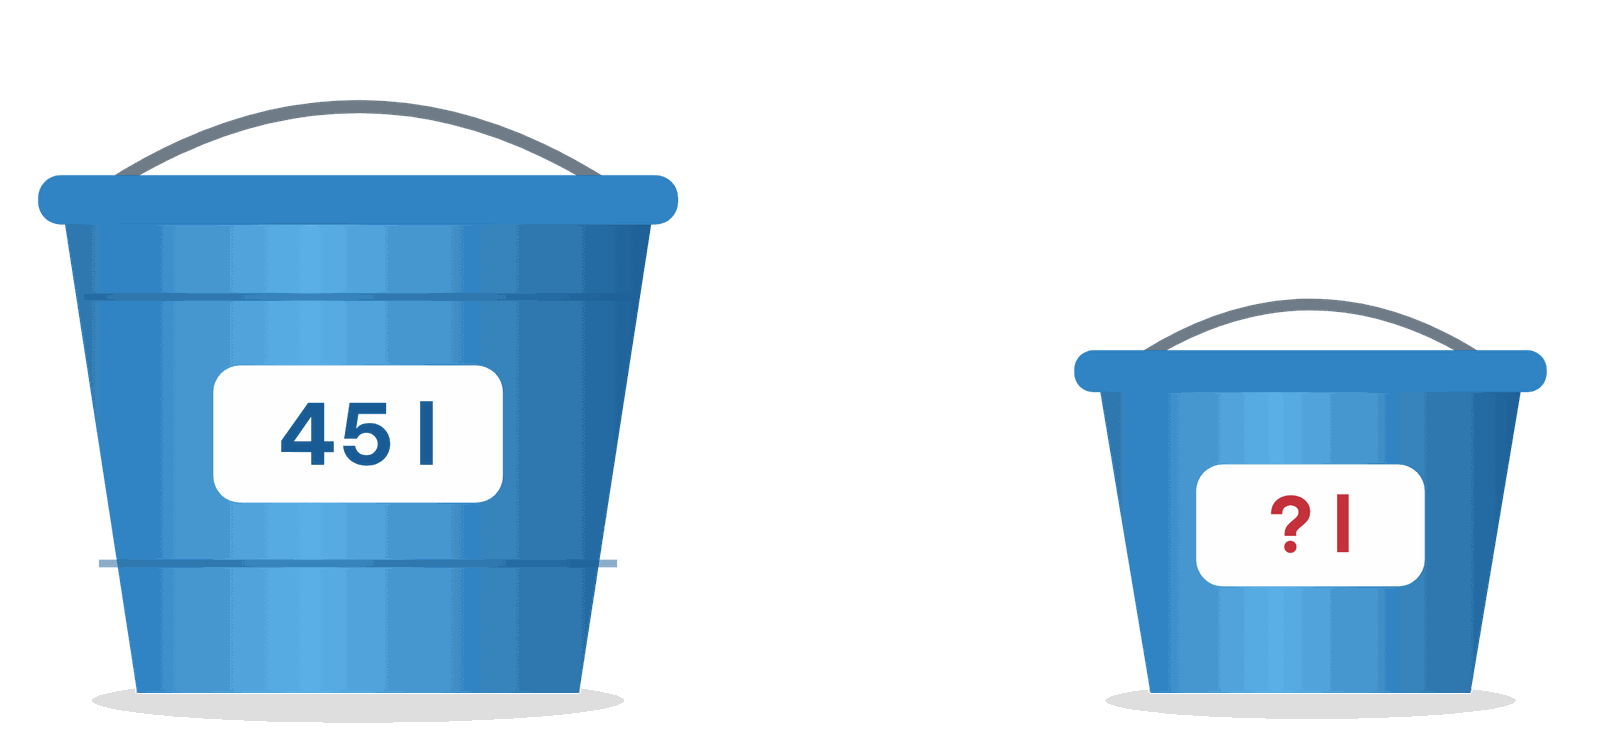
\includegraphics[width=\linewidth]{ga06_thungnuoc.png}\\[2pt]
    {\small\textit{Hình 12. Thùng to và thùng nhỏ.}}
\end{minipage}\hfill
\begin{minipage}[c]{0.53\linewidth}
    \centering
    \begin{tikzpicture}[x=0.14cm,y=1cm]
        \node[anchor=east,font=\bfseries\small] at (-1,1.5) {Thùng to};
        \node[anchor=east,font=\bfseries\small] at (-1,0) {Thùng nhỏ};
        \fill[gaBangGiay,rounded corners=2pt] (0,1.35) rectangle (45,1.65);
        \fill[gaBangGiay,rounded corners=2pt] (0,-0.15) rectangle (33,0.15);
        \draw[gaDo,densely dashed,thick,rounded corners=2pt] (33,-0.15) rectangle (45,0.15);
        \foreach \x in {0,45}{\draw[thick] (\x,1.25) -- (\x,1.75);}
        \foreach \x in {0,33}{\draw[thick] (\x,-0.25) -- (\x,0.25);}
        \draw[densely dashed] (45,1.25) -- (45,0.15);
        \node[gaTim,above] at (22.5,1.75) {45 l};
        \node[gaDo,above] at (39,0.2) {12 l};
        \draw[thick] (0,-0.35) to[out=-90,in=180] (0.8,-0.55) -- (15.7,-0.55) to[out=0,in=90] (16.5,-0.75) to[out=90,in=180] (17.3,-0.55) -- (32.2,-0.55) to[out=0,in=-90] (33,-0.35);
        \node[gaTim,below] at (16.5,-0.75) {? l};
    \end{tikzpicture}\\[2pt]
    {\small\textit{Hình 13. Thùng nhỏ bằng thùng to bớt đi đoạn 12 l (nét đứt).}}
\end{minipage}
\GAvo{\centerline{\underline{Bài giải}}
\hspace*{2em}Thùng nhỏ đựng số lít nước là:\\
\hspace*{4em}$45 - 12 = 33$ (l)\\
\hspace*{6em}Đáp số: 33 l nước.}
\GAmucnho{Luyện tập trong PBT: Bài 8, Bài 9, Bài 10}
Bài 8: HS điền số vào sơ đồ cho sẵn; Bài 9: HS tự vẽ sơ đồ vào khung rồi giải.
\begin{enumerate}[a)]
    \item[\textbf{Bài 8.}] Tổ Một trồng được 26 cây. Tổ Hai trồng được nhiều hơn tổ Một 7 cây. Hỏi tổ Hai trồng được bao nhiêu cây? \hfill ($26 + 7 = 33$)
    \item[\textbf{Bài 9.}] Anh cao 95 cm. Em thấp hơn anh 18 cm. Hỏi em cao bao nhiêu xăng-ti-mét? \hfill ($95 - 18 = 77$)
\end{enumerate}
\textbf{Bài 10 (HS khá giỏi).} Nhìn sơ đồ (thùng cam 40 quả, thùng quýt ít hơn thùng cam 15 quả), HS nêu bài toán rồi giải. \GAdapan{Thùng quýt có số quả là: $40 - 15 = 25$ (quả)}\par
\begin{luuy}
    \begin{itemize}
        \item Đề hỏi về ai thì câu lời giải nói về người đó: hỏi “Hoa có\dots” thì viết “Hoa có số cái nhãn vở là:”.
        \item “Thấp hơn”, “nhẹ hơn”, “ngắn hơn” cũng là dạng ít hơn; “cao hơn”, “nặng hơn”, “dài hơn” là dạng nhiều hơn.
        \item Phân hóa: HS giỏi làm thêm bài toán ngược ở phần từ khóa (Lan có 32, Lan nhiều hơn Hoa 9 $\Rightarrow$ Hoa có $32 - 9 = 23$).
    \end{itemize}
\end{luuy}

%---------------------------------------------------------
\subsubsection{TRÒ CHƠI “RUNG CHUÔNG VÀNG” -- CỦNG CỐ -- GIAO BÀI TẬP VỀ NHÀ}
\begin{hd}
    \begin{itemize}
        \item Thời gian: 15 phút
        \item HS vận dụng nhanh cả 3 dạng toán; tự nhắc lại khi nào làm phép cộng, khi nào làm phép trừ.
    \end{itemize}
\end{hd}
\noindent\begin{minipage}[c]{0.18\linewidth}
    \centering
\includegraphics[width=0.9\linewidth]{ga06_chuong.png}
\end{minipage}\hfill
\begin{minipage}[c]{0.79\linewidth}
    Cả lớp ngồi tại chỗ với bảng con. GV đọc từng câu (chiếu lên TV), HS có 30 giây để viết \textbf{phép tính và kết quả}. Sai thì tạm dừng chơi; sau câu 3, GV “cứu trợ” cả lớp bằng một câu hỏi lí thuyết. Bạn trả lời đúng câu 6 được rung chuông vàng.
\end{minipage}
\begin{vd}
    \begin{enumerate}
        \item Có 14 quả bóng xanh và 5 quả bóng đỏ. Hỏi có tất cả bao nhiêu quả bóng? \hfill ($14 + 5 = 19$)
        \item Có 20 cái bánh, cả nhà đã ăn 8 cái. Hỏi còn lại bao nhiêu cái bánh? \hfill ($20 - 8 = 12$)
        \item Nhà bác Hai nuôi 35 con gà, số vịt nhiều hơn số gà 10 con. Hỏi nhà bác nuôi bao nhiêu con vịt? \hfill ($35 + 10 = 45$)
        \item Bút chì dài 16 cm, bút mực ngắn hơn bút chì 3 cm. Hỏi bút mực dài bao nhiêu xăng-ti-mét? \hfill ($16 - 3 = 13$)
        \item Xe buýt có 30 hành khách, đến bến có 12 người xuống xe. Hỏi trên xe còn bao nhiêu hành khách? \hfill ($30 - 12 = 18$)
        \item \textbf{Câu chuông vàng:} Hộp thứ nhất có 27 viên bi. Hộp thứ hai có nhiều hơn hộp thứ nhất 8 viên. Hỏi cả hai hộp có bao nhiêu viên bi? \hfill ($27 + 8 = 35$; $27 + 35 = 62$)
    \end{enumerate}
\end{vd}
\begin{itemize}
    \item \textbf{Củng cố (3 phút):} \GAloi{Khi nào con làm phép cộng? Khi nào con làm phép trừ?} HS trả lời bằng lời của mình; GV chốt lại 4 bước trên bảng trái.
    \item Đếm vé xe buýt, đổi sticker; nhắc nhở HS còn quên viết đơn vị hoặc đáp số.
    \item \textbf{BTVN:}
\end{itemize}
\textbf{Bài 11.} Nhà bác Ba nuôi 42 con gà. Bác bán đi 15 con. Hỏi nhà bác Ba còn lại bao nhiêu con gà? \GAdapan{$42 - 15 = 27$ con}\par
\textbf{Bài 12.} Bao gạo thứ nhất nặng 35 kg. Bao gạo thứ hai nặng hơn bao thứ nhất 18 kg. Hỏi bao gạo thứ hai nặng bao nhiêu ki-lô-gam? \GAdapan{$35 + 18 = 53$ kg}\par
\textbf{Bài 13.} Con hãy nhìn đồ vật trong nhà (đôi dép, quả trong tủ lạnh, sách trên giá, \dots), tự đặt một đề toán có lời văn rồi giải. Buổi sau đọc đề cho cả lớp cùng giải.

\begin{center}
       \faGg\faGg\quad Hết \quad\faGg\faGg
\end{center}
\end{document}
